% SLIDE GENERATION INSTRUCTIONS

% For each slide I will paste in latex code with comments.
% For each comment, identify how to best address it
% considering the other comments and the context from the paper.

% To address each comment, ONLY write the changes you propose
% in code blocks I can easily paste into the latex document.
% For each code block explain HOW your changes address my comments.
% Think step-by-step and always identify your previous issues first.
% Make sure to output latex that is at most 80 chars per line,
% make plenty line breaks to ensure good readability.

% When writing slides, please make sure to keep this logical
% structure so that it is still understandable.
% It must have a narrative, that is very important.
% Split one 'slide' into multiple pages using the package and
% \only<slide number, e.g. 1, 2 or even '1-2' for both> {..} to make it more easy to follow
% for listeners.

% Your output should look like this:
% ## Slide <num>: <slide title>
% This slide addresses the comment <comment from latex> by
% <one sentence explanation of slide contents>.
% ```latex
% \only<1> { % Slide 1 content, narrative, etc. }
% \only<2-3> { % Slide 2, transition to 3 }
% \only<3> { % Slide 3 content, narrative, etc. }
% ```

\documentclass{beamer}
\usetheme{Madrid} 
\usepackage{graphicx}
\usepackage{hyperref}
\usepackage{tikz}
\usepackage{pgfplots}
\usetikzlibrary{positioning}

\title{Nonsmooth Optimization via Quasi-Newton Methods}
\author{Adrian S. Lewis and Michael L. Overton}
\date{}

\begin{document}

\begin{frame}
    \titlepage
\end{frame}

\begin{frame}{Outline}
    \tableofcontents
\end{frame}

\section{Introduction}
\begin{frame}{Basics of Optimization}
    % Slide 1: Define Optimization Problem
    % Slide 2: Write out Taylor Approximation
    % Slide 3: Explain Gradient Descent

    \only<1> {
        The general unconstrained optimization problem
        is given by:
        \begin{equation*}
            \min_{x \in \mathbb{R}^n} f(x),
        \end{equation*}
        where $f: \mathbb{R}^n \to \mathbb{R}$ is a
        twice-differentiable real-valued function.
    }

    \only<2-3> {
        % First-order Taylor approximation
        The first-order Taylor approximation
        of $f$ around $x_k$ yields:
        \begin{align*}
            f(x) & \approx f(x_k) + \nabla f(x_k)^T (x - x_k).
        \end{align*}
    }

    \only<3> {
        Which motivates the Gradient Descent method as follows:
        \begin{align*}
            x_{k+ 1} = x_k - t_k \nabla f(x_k),
        \end{align*}
        where $t_k > 0$ is some step size.
    }
\end{frame}

\begin{frame}{Newton's Method}
    \only<1-2> {
        % Second-order taylor approximation
        The second-order Taylor approximation of $f$ around $x_k$ yields:
        \begin{align*}
            f(x) & \approx f(x_k) + \nabla f(x_k)^T (x - x_k)           \\
                 & + \frac{1}{2} (x - x_k)^T \nabla^2 f(x_k) (x - x_k).
        \end{align*}
        A necessary condition for a local minimizer $x_k$
        is that $\nabla f(x_k) = \mathbf{0}$.
    }

    \only<2> {
        % Also from Taylor Approximation
        \vspace{0.5em}
        `Jumping' to the minimizer of this quadratic
        approximation yields Newton's Method:
        \begin{align*}
            x_{k+1} = x_k - (\nabla^2 f(x_k))^{-1} \nabla f(x_k),
        \end{align*}
        where $\nabla^2 f(x_k)$ is the Hessian matrix.
    }
\end{frame}

\section{Quasi-Newton Methods}
\begin{frame}{Quasi-Newton Methods}
    % Define QN method as in the paper
    \only<1> {
        The main disadvantage of Newton's method
        is the need to compute
        the Hessian matrix $\nabla^2 f(x_k) \in \mathbb{R}^{n \times n}$
        and solve a linear system of equations
        in every iteration.

        \vspace{0.5em}
        Also, the true Hessian might not always be positive definite.
    }

    \only<2> {
        Quasi-Newton methods approximate the
        \textbf{inverse} Hessian
        $$H_k \approx (\nabla^2 f(x_k))^{-1}$$
        by iteratively updating $H_k$.
    }

    \only<3> {
        \begin{block}{Algorithm 2.1 (quasi-Newton method)}
            Choose $x_0$ with $f$ differentiable at $x_0$,
            set $H_0$ to a positive definite matrix and
            $k \leftarrow 0$

            \texttt{repeat}

            \qquad compute search direction $p_k \leftarrow -H_k \nabla f_k$

            \qquad set $x_{k + 1} \leftarrow x_k + t_k p_k$,
            where $t_k > 0$ \\
            \qquad\qquad is chosen by a line search

            \qquad \texttt{if} $f$ is not differentiable at $x_{k + 1}$,
            or $\nabla f_{k + 1} = 0$, \\
            \qquad\qquad stop.

            \qquad set $y_k \leftarrow \nabla f_{k + 1} - \nabla f_k$

            \qquad choose $H_{k + 1}$ to be a positive definite matrix
            satisfying \\
            \qquad\qquad the secant condition $H_{k + 1} y_k = t_k p_k$

            \qquad $k \leftarrow k + 1$

            \texttt{end (repeat)}
        \end{block}
    }

    \only<4> {
        The true Hessian has the property
        \begin{align*}
            \nabla^2 f(x_{k}) \underbrace{
                (x_{k + 1} - x_k)
            }_{t p_k} =
            \underbrace{
                \nabla f(x_{k + 1}) - \nabla f(x_k)
            }_{y_k},
        \end{align*}
        by the Taylor expansion of $\nabla f$ at $x_k$,
        which results in the secant equation since
        $H_{k + 1} \approx (\nabla^2 f(x_k))^{\mathbf{-1}}$.
    }

    % Clarify a number of things from the algorithm
    \only<5> {
        The BFGS algorithm updates the inverse Hessian using:
        \begin{align*}
            H_{k + 1} & = V_k H_k V_k^T + t_k \frac{
                p_k p_k^T
            }{p_k^T p_k}                                   \\
            V_k       & = I - \frac{p_k y_k^T}{p_k^T y_k}.
        \end{align*}
    }
\end{frame}

\begin{frame}{Non-smooth Optimization}
    % Illustrate Problem of GD in non-smooth optimization, e.g. Abs value
    \only<1> {
        \begin{figure}
            % Abs value plot
            \begin{figure}
                \centering
                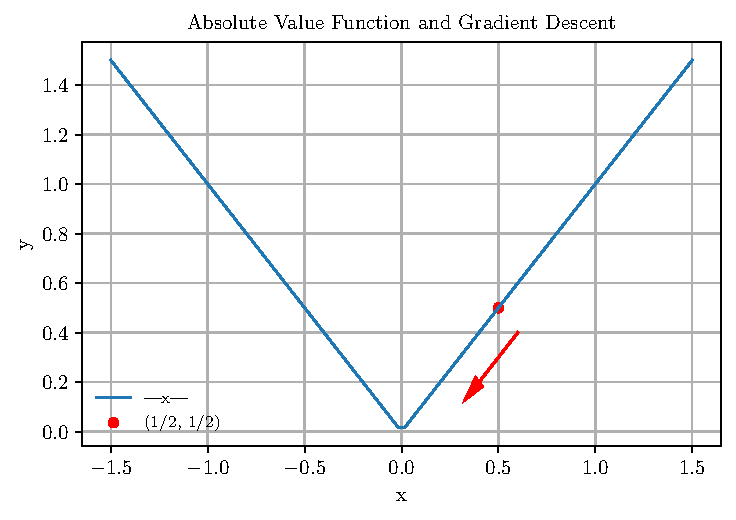
\includegraphics[width=0.7\textwidth]{plots/abs_val_func.pdf}
                \caption{The absolute value function and Gradient Descent
                    with $x_0 = \frac{1}{2}$ and $t_k = 1$.}
                \label{fig:abs_value_function}
            \end{figure}
        \end{figure}
    }

    \only<2> {
        The problem is that the gradient does not smoothly change
        near the minimum, but jumps from $-1$ to $1$.
        The gradient is not continuous at the minimum.
    }

    \only<3> {
        In fact, with \textbf{any constant step size} $t_k$,
        Gradient Descent will oscillate forever on this problem.
    }
\end{frame}

\subsection{Line Search}
\begin{frame}{Exact Line Search}
    % Define exact line search
\end{frame}

\begin{frame}{Armijo-Wolfe Conditions}
    % Define Armijo-Wolfe Conditions
    % Illustrate with plot
\end{frame}

\begin{frame}{Inexact Line Search}
    % Define Armijo-Wolfe Conditions
\end{frame}

\section{Numerical Experiments}
\begin{frame}{Optimization Example on Euclidean Norm Function}
    % Euclidean norm plot
    \begin{figure}
        \centering
        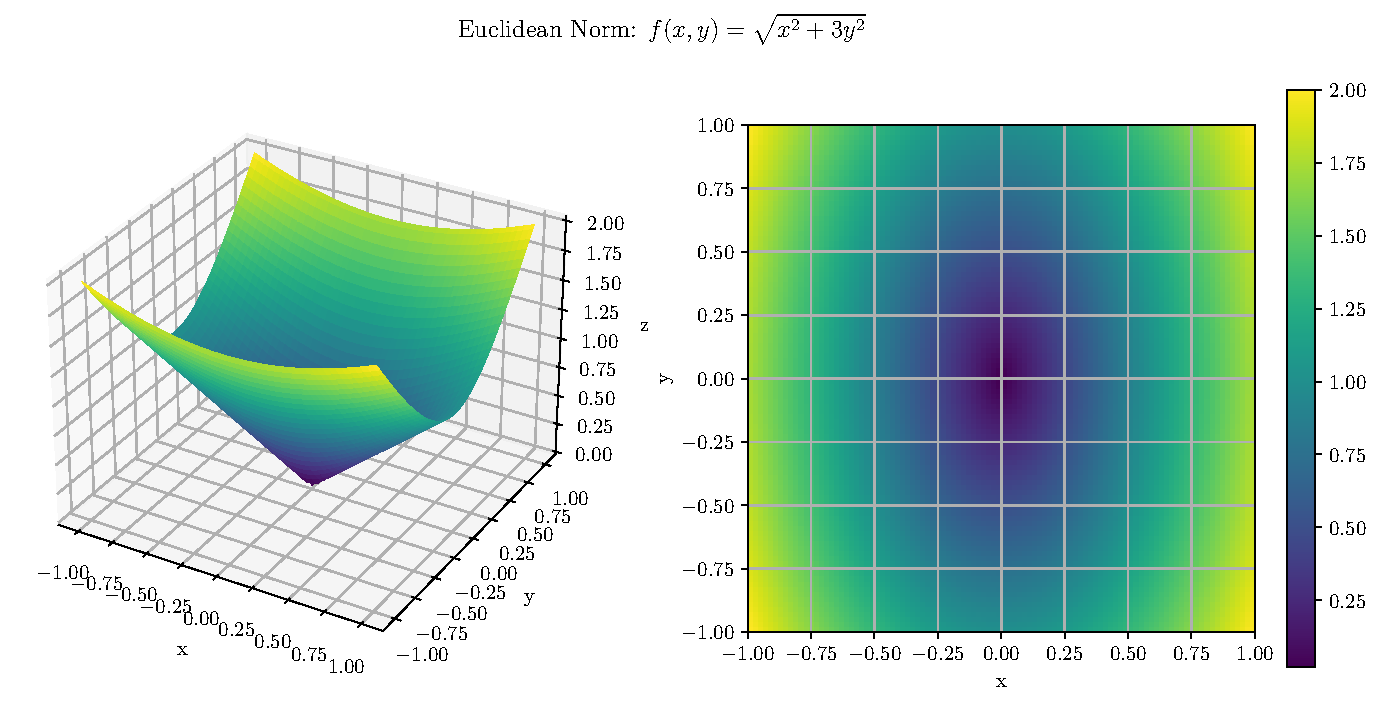
\includegraphics[width=1.0\textwidth]{plots/euclidean_norm.pdf}
        \caption{The (skewed) Euclidean norm function}
        \label{fig:euclidean_norm_function}
    \end{figure}
\end{frame}

\section{Conclusion}
\begin{frame}{Conclusion}
    % Summarize the paper
\end{frame}

\end{document}